%this file is the first report
%a % comment anything after % until the end of the line

%minimum references to begin our article
\documentclass[12pt]{article}
\usepackage[frenchb]{babel}
\usepackage[utf8]{inputenc}
\usepackage[T1]{fontenc}
\usepackage{graphicx}
\usepackage{fancyhdr}
\usepackage{hyperref}
\usepackage{float}
\usepackage{amsmath}
\usepackage[margin=1in]{geometry}
\usepackage{indentfirst}


\pagestyle{fancy}
%\cfoot{Insattack : Projet de POO}
% the last extension makes it possible to add images

%presentation of the document
\title{Insattack : Projet de POO\smallbreak Rapport de conception}
\author{Baptiste \textsc{Bignon}, Gabriel \textsc{Prevosto}}
\date{12/11/2014}
\setlength\parindent{15pt}
\begin{document}

\maketitle
%\begin{figure}[!h] 
%\centerline{\includegraphics[scale=0.50]{img/arimaa}}
%\end{figure}
\newpage

%to add a table of contents
\tableofcontents
\renewcommand{\contentsname}{Sommaire}
\newpage


\section{Introduction}			\label{sec:introduction}
\newpage

\section{Le jeu}				\label{sec:jeu}
\subsection{Les règles}			\label{sec:regles}
\subsection{Les peuples}			\label{peuples}
\subsection{Les terrains}			\label{terrains}
\newpage

\section{Architecture}			\label{sec:archi}
\subsection{Architecture principale}	\label{sec:architecturePrincipale}
\subsection{Création d'une partie}	\label{sec:creationPartie}
\subsection{Déroulement d'une partie}	\label{sec:deroulementPartie}
\subsection{Cycle de vie des unités}	\label{sec:cycleVieUnites}
\newpage

\section{Implémentation}			\label{sec:implementation}
\subsection{Diagramme de classes}	\label{sec:diagrammeClasses}		Dans le cadre de l'étape de conception, un diagramme de classes représentant le modèle du jeu a été réalisé.

\begin{figure}[!h]
\centering
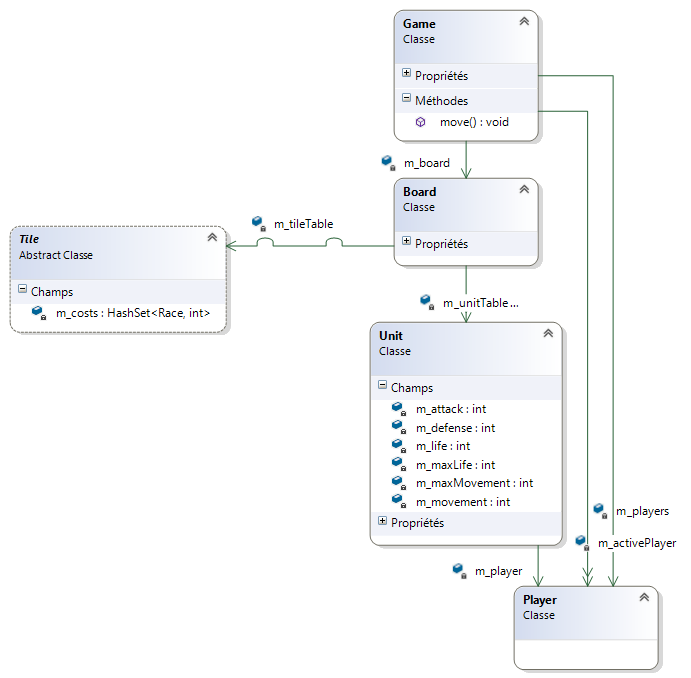
\includegraphics[width=\textwidth]{Parties/Images/UML_Princ.png}
\caption{Les classes princpales de la représentation du jeu}
\label{fig:uml_princ}
\end{figure}

Chaque joueur est reporésenté par une instance de la classe \emph{Player}.
La classe \emph{Board} contiendra le terrain (sous forme d'instances de \emph{Tile}), ainsi que les unités (instances de \emph{Unit}).
La classe \emph{Game} contiendra le plateau, et sera capable d'appliquer les règles du jeu.
\subsection{Patrons de Conception}	\label{sec:patronsConception}		Afin de faciliter l'implémentation et rendre le projet plus facilement compréhensible, des patrons de conception ont été implémentés.
Ces derniers seront explicités dans les parties qui suivent.

\subsubsection{Création des départements} %Fabrique

\begin{figure}[!h]
\centering
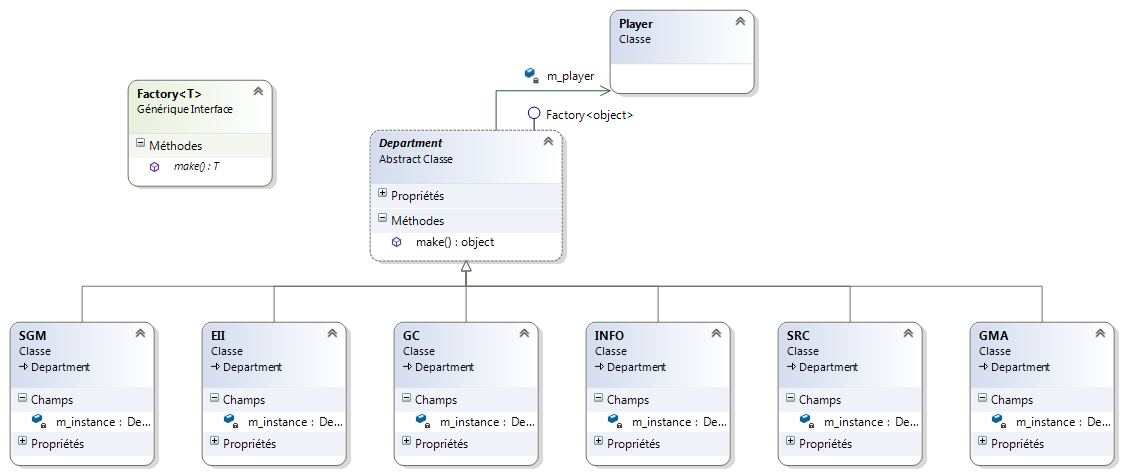
\includegraphics[width=\textwidth]{Parties/Images/UML_Dept.png}
\caption{Patron fabrique appliqué aux dépatements}
\label{fig:uml_dept}
\end{figure}

Le patron de conception \emph{fabrique} permet de créer des objets sans connaître leur classe, et éventuellement d'effectuer des opérations supplémentaires à la création.
Appliqué aux départements, elle permet à ces derniers de créer des unités qui leur sont spécifiques.
Par exemple, la méthode \emph{make()} du département \emph{INFO} ne créera pas les mêmes unités que celle du département \emph{EII}.

\subsubsection{Création d'une partie} %Monteur

\begin{figure}[!h]
\centering
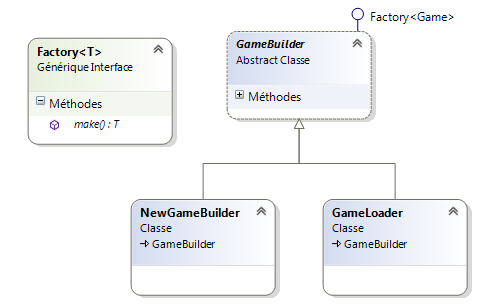
\includegraphics[width=0.5\textwidth]{Parties/Images/UML_Game.png}
\caption{Patron monteur appliqué à la création de parties}
\label{fig:uml_game}
\end{figure}

Le patron de conception \emph{monteur} permet de créer des objets suivant différents scénarios.
Ici, par exemple, on pourra créer une nouvelle partie ou charger une partie sauvegardée.

\subsubsection{Modélisation du terrain} %Poids-mouche

\begin{figure}[!h]
\centering
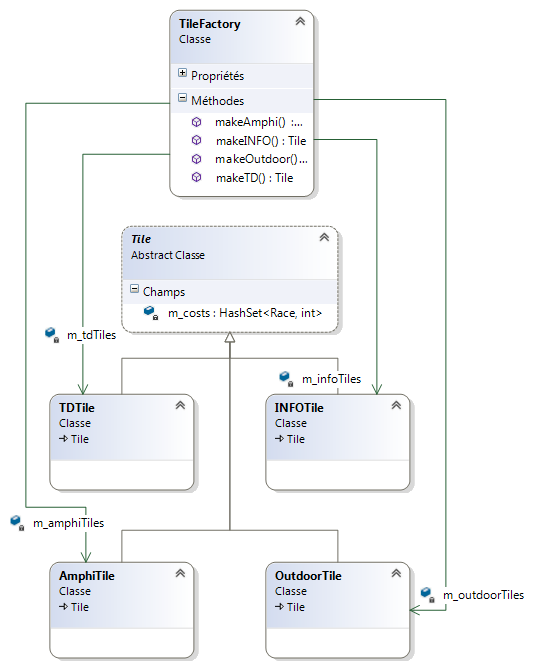
\includegraphics[width=0.5\textwidth]{Parties/Images/UML_Tiles.png}
\caption{Patron poids-mouche appliqué au terrain}
\label{fig:uml_tiles}
\end{figure}

Le patron de conception \emph{poinds-mouche} permet de contrôler le nombre d'instances d'un objet.
Dans le cas du terrain, chaque type de case (classes héritant de \emph{Tile}) ne sera instanciée qu'une fois.
Par exemple, les différentes salles informatiques pointeront vers la même instance de \emph{INFOTile}.

\subsubsection{Création de différents types de carte} %Stratégie

\begin{figure}[!h]
\centering
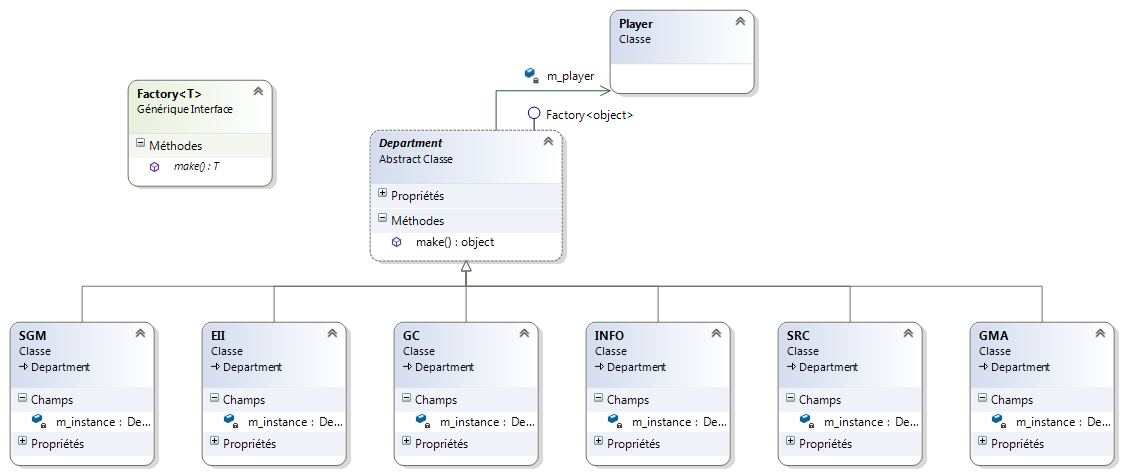
\includegraphics[width=\textwidth]{Parties/Images/UML_Dept.png}
\caption{Patron stratégie appliqué à la création des cartes}
\label{fig:uml_board}
\end{figure}

Le patron de conception \emph{stratégie} permet de réaliser une opération de différentes manières.
Ici, il s'agit de créer différents types de cartes de différentes tailles.
\newpage

\section{Conclusion} 			\label{sec:conclusion}			La conception du modèle pour le jeu \emph{Insattack} est finie, son implémentation peut donc commencer.
L'interface utilisateur n'a pas encore été pensée ; cependant, le modèle n'y fait pas référence et peut donc être développé avant.
Par la suite, l'interface graphique utilisera le modèle pour gérer la partie.

Les règles du jeu ont été légèrement modifiées afin de correspondre avec l'environnement de l'INSA ; il sera donc peut-être nécessaire de les modifier à nouveau dans un souci d'équilibrage.
Cependant, ces modifications seront simples à effectuer grâce à l'utilisation des patrons de  conception décrits dans la partie \ref{sec:patronsConception}.


\end{document}
